\documentclass[cn]{elegantpaper}
\author{邵李翔\quad 赵张弛 \quad 祖劭康}
\title{线性回归,岭回归以及Lasso回归}
\date{}
\usepackage{float}
\begin{document}
    
\maketitle
\begin{abstract}
  我们采用Boston数据集,使用线性回归、lasso、岭回归三种方式进行建模,以数据集中的medv变量为响应变量,其余13个变量为预测变量,探究之间的线性关系。并比较三种模型求解出来的系数,分析三种方法的优缺点。
\end{abstract}
\section{数据集描述}
本次实验采用的数据集为Boston (波士顿房价)数据集,它记录了波士顿周围 506 个街区的 medv
(房价中位数)。我们将设法用 13 个预测变量如 rm (每栋住宅的平均房间数), age (平均房
龄), lstat (社会经济地位低的家庭所占比例)等来预测 medv (房价中位数)。下表是部分数据集展示。
\begin{table}[ht]
    \centering
    \caption{数据集中部分数据展示}
    \begin{tabular}{rrrrrrrrrrrrrrr}
      \hline
     & crim & zn & indus & chas & nox & rm & age & dis & rad & tax & ptratio & black & lstat & medv \\ 
      \hline
    1 & 0.01 & 18.00 & 2.31 & 0.00 & 0.54 & 6.58 & 65.20 & 4.09 & 1.00 & 296.00 & 15.30 & 396.90 & 4.98 & 24.00 \\ 
      2 & 0.03 & 0.00 & 7.07 & 0.00 & 0.47 & 6.42 & 78.90 & 4.97 & 2.00 & 242.00 & 17.80 & 396.90 & 9.14 & 21.60 \\ 
      3 & 0.03 & 0.00 & 7.07 & 0.00 & 0.47 & 7.18 & 61.10 & 4.97 & 2.00 & 242.00 & 17.80 & 392.83 & 4.03 & 34.70 \\ 
       \hline
    \end{tabular}
\end{table}

\section{线性回归}
由于最小二乘法求解线性模型参数能直接得到解析解,所以我们对所有预测变量进行多元回归,得到的结果如表2。由各个预测变量对应的系数的值可以看出来,有些变量比如black,age等系数绝对值小于0.01,可以说与响应变量——房价中位数关系不大,而且表格第五列是系数显著性检验的结果,比如indus、age对应的p值显然是表明接受原假设,认为该变量的系数应该等于0。说明线性回归在某些数据集上还存在一定的局限性。
\begin{table}[H]
    \centering
    \caption{多元线性回归拟合结果}
    \begin{tabular}{rrrrr}
      \hline
     & Estimate & Std. Error & t value & Pr($>$$|$t$|$) \\ 
      \hline
    (Intercept) & 36.4595 & 5.1035 & 7.14 & 0.0000 \\ 
      crim & -0.1080 & 0.0329 & -3.29 & 0.0011 \\ 
      zn & 0.0464 & 0.0137 & 3.38 & 0.0008 \\ 
      indus & 0.0206 & 0.0615 & 0.33 & 0.7383 \\ 
      chas & 2.6867 & 0.8616 & 3.12 & 0.0019 \\ 
      nox & -17.7666 & 3.8197 & -4.65 & 0.0000 \\ 
      rm & 3.8099 & 0.4179 & 9.12 & 0.0000 \\ 
      age & 0.0007 & 0.0132 & 0.05 & 0.9582 \\ 
      dis & -1.4756 & 0.1995 & -7.40 & 0.0000 \\ 
      rad & 0.3060 & 0.0663 & 4.61 & 0.0000 \\ 
      tax & -0.0123 & 0.0038 & -3.28 & 0.0011 \\ 
      ptratio & -0.9527 & 0.1308 & -7.28 & 0.0000 \\ 
      black & 0.0093 & 0.0027 & 3.47 & 0.0006 \\ 
      lstat & -0.5248 & 0.0507 & -10.35 & 0.0000 \\ 
       \hline
    \end{tabular}
\end{table}

\section{Lasso}
   \subsection{模型介绍}
   Lasso在基础的线性回归模型的损失函数上,增加了L1正则项,假设有p个预测变量,此时Lasso损失函数如下:
   \begin{equation}
    \sum_{i=1}^n(y_i-\beta^Tx_i)^2+\lambda\sum_{j=1}^p|\beta_j|
   \end{equation}
   这里$\lambda$是超参数。
   
    \subsection{超参数$\lambda$选择}
    调用R语言glmnet包,实现Lasso Regression,将数据分成十份,计算不同超参数$\lambda$下交叉验证(Cross Validation)的误差,并选择最优的超参数,结果如图1所示
    \begin{figure}[htbp]
        \centering
        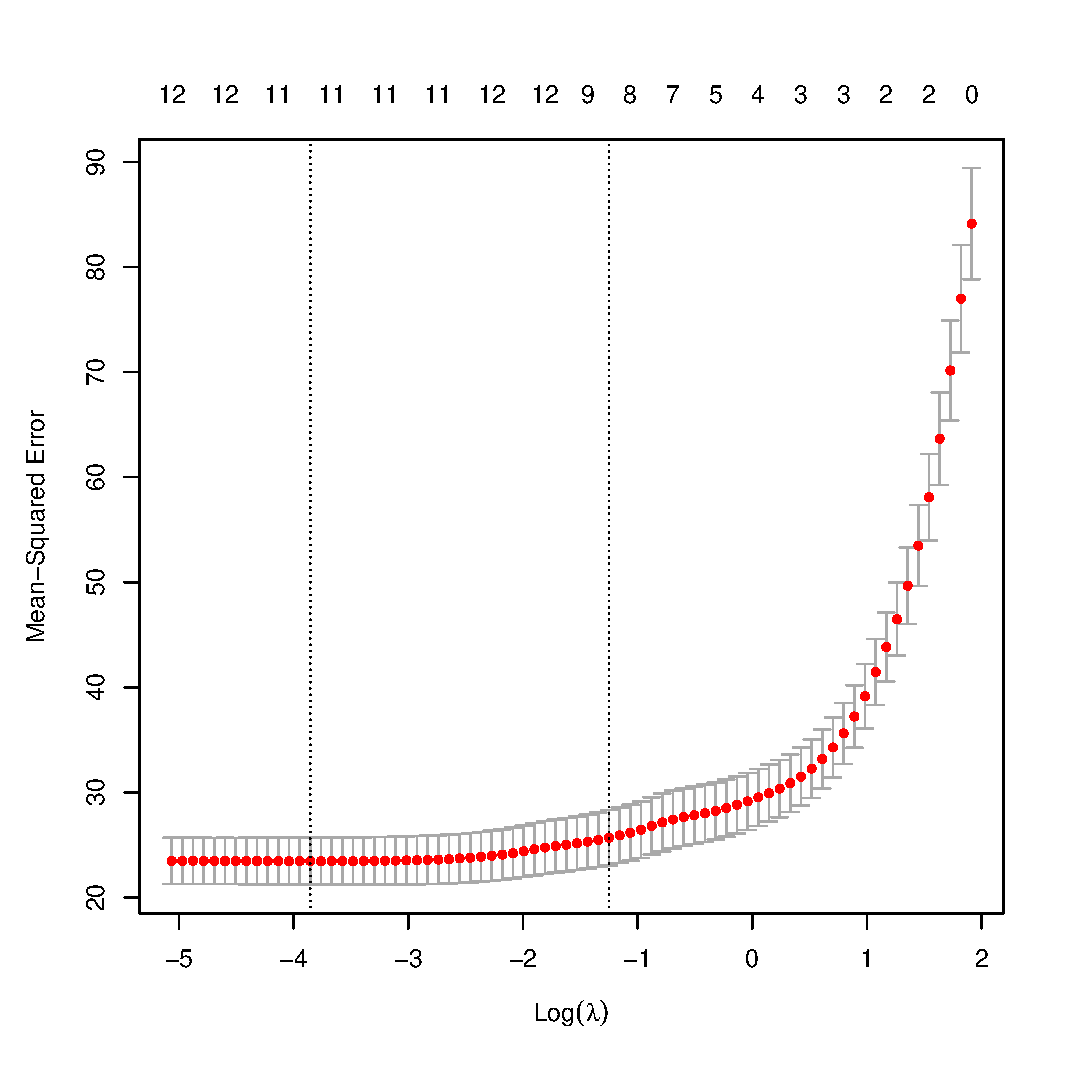
\includegraphics[width=0.6\textwidth]{lassocv.eps}
        \caption{Lasso Cross Validation}
    \end{figure}
    由结果可知,我们选取最小的均方误差对应的超参数系数,最优的$\lambda$取值约为0.021。
    \subsection{结果及分析}
    分别用glmnet包和自己编写的使用循环坐标下降法进行优化的代码在最优的$\lambda$取值下进行Lasso Regression,拟合得到的模型系数如表3所示
    \begin{table}[H]
        \centering
        \caption{自己编写与glmnet包用lasso估计系数的结果}
        \begin{tabular}{|c|c|c|c|c|c|c|c|c|c|c|c|c|c|c|}
        \hline
               & crim  & zn   & indus & chas & nox    & rm   & age  & dis   & rad  & tax   & ptratio & black & lstat & intercept \\ \hline
        glmnet & -0.10 & 0.04 & 0.00  & 2.69 & -16.57 & 3.85 & 0.00 & -1.42 & 0.26 & -0.01 & -0.93   & 0.01  & -0.52 & 34.91     \\ \hline
        ours   & -0.10 & 0.02 & -0.02 & 4.45 & -11.34 & 3.41 & 0.00 & -0.75 & 0.00 & 0.00  & 0.00    & 0.00  & -0.55 & 17.16     \\ \hline
        \end{tabular}
    \end{table}
    从表中我们可以看出,glmnet包的结果与我们的结果在各个项与房价的正负相关性上是相同的,但我们的结果将更多的系数压缩到0。存在这种差别的原因是lasso无法得到系数解析解,所以要采用别的计算方法,而我们优化计算系数的方式是循环坐标下降法,而R自带包计算系数的方法是最小角回归法,计算方法上最小角回归法更容易得到最优解。但两种方法的结果总体比较还是较为一致的。
    
    在glmnet的结果中,房价与crim犯罪率、nox氮氧化物浓度、dis到就业中心的距离、ptratio学生与教师比例、lstat人口数量呈负相关,与zn住宅用地比例、chas查尔斯河虚拟变量、rm每栋住宅的平均房间数、rad可达公路数、black黑人比例呈正相关,与indus、age两个变量无关,而这也与之前线性回归模型参数估计中,发现这两个变量的系数显著性检验并未通过的结果相一致。

    在我们的结果中。房价与犯罪率、indus商场面积、氮氧化物浓度、到就业中心的距离、人口数量呈负相关,与住宅用地比例、查尔斯河虚拟变量、每栋住宅的平均房间数呈正相关,与其余变量无关。

    以上结果都与常识相符,比如犯罪率与房价的负相关性。接下来我们比较超参数一致情况下,两种方式计算的MSE结果,两种代码的MSE如下表所示
    \begin{table}[H]
        \centering
        \caption{采用自己编写与glmnet包的系数计算的MSE比较}
        \begin{tabular}{|c|c|}
        \hline
               & MSE   \\ \hline
        glmnet & 21.92 \\ \hline
        ours   & 27.72 \\ \hline
        \end{tabular}
    \end{table}
    由结果可见,glmnet包训练的模型MSE更小,但是我们的循环坐标下降法本身选择的有效变量更少(系数非零的变量个数少),这样也会导致MSE增加,所以MSE不是一个很好的比较标准,但是采用最小角回归方法优化计算的lasso系数估计值更与线性回归的结果一致。

\section{岭回归}
\subsection{模型介绍}
岭回归是在基础的线性回归模型的损失函数上,增加了L2正则项,同样假设有p个预测变量,此时Lasso损失函数如下:
\begin{equation}
 \sum_{i=1}^n(y_i-\beta^Tx_i)^2+\lambda\sum_{j=1}^p\beta_j^2
\end{equation}
由于岭回归的损失函数可导,所以也可以直接求解出一个回归系数的估计值为$\hat{\beta}=(X^TX+\lambda I)^{-1}XY$,随着 $\lambda$的增大,$(X^TX+\lambda I)^{-1}$就越小,模型的方差就越小;而$\lambda$越大使得 $\beta$的估计值更加偏离真实值,模型的偏差就越大。所以岭回归的关键是找到一个合理的 $\lambda$值来平衡模型的方差和偏差。

\subsection{自己实现的岭回归与自带包实现的岭回归}
这里我们先比较自己实现的岭回归的参数估计与自带包实现的参数。首先选取超参数$\lambda$为$0.01$,使用两种不同的代码实现岭回归,得到模型中的参数如下表。我们可以看到两者系数相差无几,而之前lasso自己编写的代码和自带包估计的系数差距较大,我们分析认为是岭回归同样能得到模型的解析解,可以直接用数据来计算得到每个超参数下系数的最优估计,所以在岭回归方面,我们自己编写的岭回归参数估计与R中自带包计算的效果几乎相同。

\begin{table}[htbp]
\centering
\caption{自己编写与R包用岭回归方法估计系数的结果}
\begin{tabular}{ccccccccccccccc}
  \hline
 & 截距项 & crim & zn & indus & chas & nox & rm & age & dis & rad & tax & ptratio & black & lstat \\ 
  \hline
  手写代码 & 35.96 & -0.11 & 0.05 & 0.02 & 2.69 & -17.48 & 3.83 & 0.00 & -1.47 & 0.30 & -0.01 & -0.95 & 0.01 & -0.52 \\ 
  自带包& 36.46 & -0.11 &  0.05 &  0.02  & 2.69 &-17.76 &3.81  & 0.00&  -1.48&   0.31 & -0.01&  -0.95&0.01&-0.52\\
   \hline
\end{tabular}
\end{table}

\subsection{基于交叉验证选择最佳参数}

自动选择参数$\lambda$值的范围进行岭回归,选择在 $\lambda =10^{-3}$到 $\lambda = 10$的范围内进行岭回归,如图所示可得每个变量的系数随着参数$\lambda$变化所得到的曲线.该图上方的13是系数个数,而下方10,15,20,25是每个$\lambda$的值对应的各变量参数的绝对值之和。我们可以从图的左端看出,即使各个变量系数的值都接近到0,但在图像上方对应的值仍为13,说明岭回归没有变量选择的作用,只会随着$\lambda$值增加,而压缩各变量系数的值。
\begin{figure}[htbp]
  \centering
  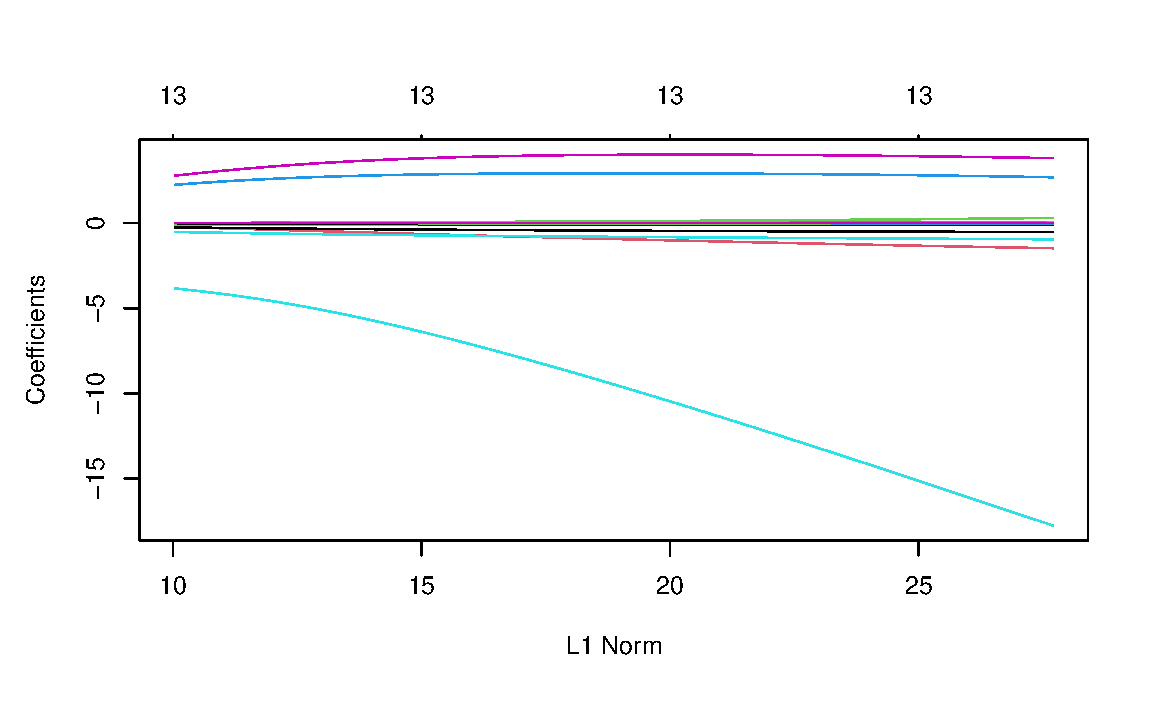
\includegraphics[width=0.8\textwidth]{opt_para.eps}
  \caption{系数变化曲线}
\end{figure}

将数据分为10折,使用交叉验证法选择调节参数$\lambda$,得到系数变化曲线如图3所示
\begin{figure}[htbp]
  \centering
  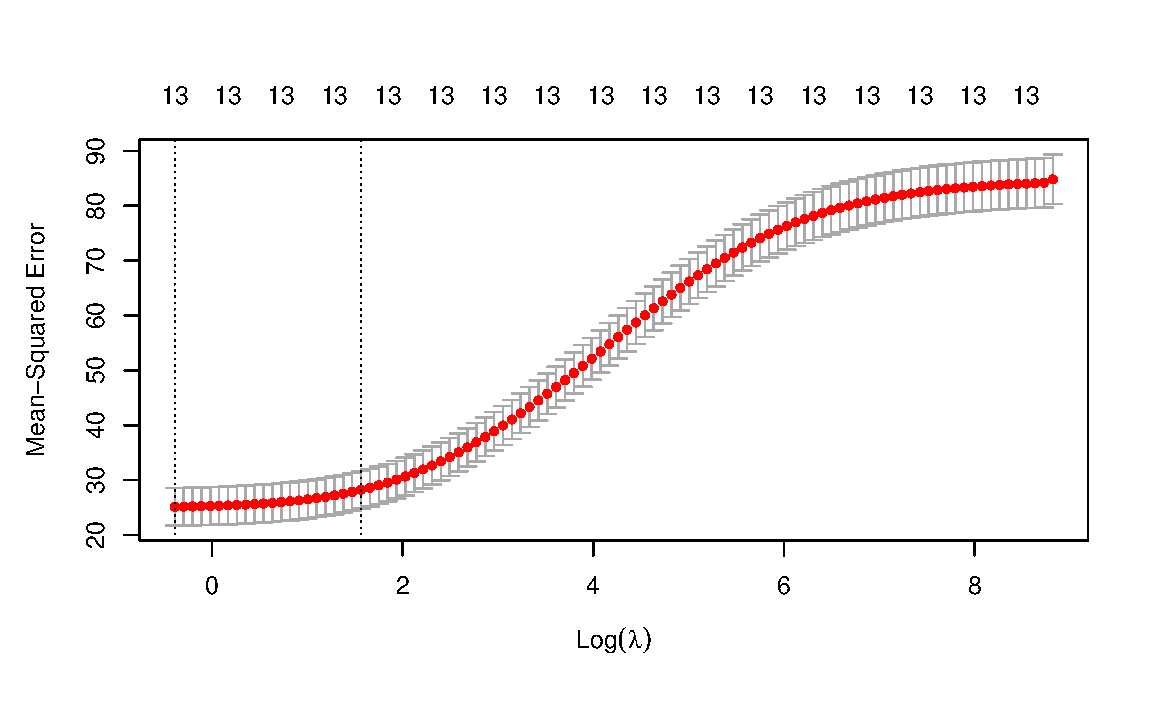
\includegraphics[width=0.6\textwidth]{cv_para.eps}
  \caption{交叉验证法的系数变化曲线}
\end{figure}

我们分别选取$\lambda$的LSE值以及最小的$\lambda$值下的变量系数,结果如图4所示,数据第一列是$\lambda$的LSE值对应的变量系数,第二列是CV准则下最小MSE的$\lambda$值下的变量系数。
\begin{figure}[htbp]
  \centering
  \includegraphics[width=0.6\textwidth]{coef.jpg}
  \caption{两个$\lambda$值下的系数}
\end{figure}


\section{总结}
对于Boston数据集直接采用线性回归进行参数估计效果并不好,我们分别采用lasso回归与岭回归方法同样对该数据集进行参数估计,lasso具有变量选择的效果,而且基于最小角回归算法得到的lasso估计参数比我们自己采用循环坐标下降法计算得到的参数效果好。而岭回归具有压缩系数的作用,但无法将系数压缩到0。




\end{document}

